\documentclass{article}

\usepackage[utf8]{inputenc}
\usepackage[T1]{fontenc}
\usepackage[greek,english]{babel}
\usepackage{alphabeta}
\usepackage{amsmath}
\usepackage{amssymb}
\usepackage{graphicx}
\usepackage{subcaption}
\usepackage{epstopdf}
\usepackage[margin=1in, paperwidth=7.5in,paperheight=10.5in]{geometry}
\usepackage{hyperref}
\usepackage{paracol}

\newcommand\course{ΗΡΥ 411}
\newcommand\courseName{Ενσωματωμένα Συστήματα Μικροεπεξεργατών}
\newcommand\semester{Χειμερινό 2020-2021}
\newcommand\assignmentNumber{Εργαστήριο 6}
\newcommand\studentName{Μαυρογιώργης Δημήτρης}                           
\newcommand\studentNumber{2016030016}

\title{\underline{\textbf{\assignmentNumber}}} 
\author{\textsc{\textbf{Όνομα:}}  \studentName\\
		\textsc{\textbf{ΑΜ:}}  \studentNumber\\
		\course \ - \courseName\\ 
		\textsc{Πολυτεχνείο Κρήτης}
		}
\date{\today}
\begin{document}
	\maketitle

\section*{Σκοπός}
	Σκοπός του έκτου εργαστηρίου είναι να κατανοήσουμε την χρησιμότητα και τη λειτουργία του watchdog timer και ειδικότερα γιατί μας είανι αρκετά χρήσιμος για τη λειτυοργία του warm start. \\

\section*{Περιγραφή της υλοποίησης}
	Πιο συγκεκριμένα, warm start είναι η διαδικασία εκκίνησης ενός υπολογιστή χωρίς να πειραχτούν-διαγραφούν τα δεδομένα από την κύρια μνήμη. Αντίθετα, cold start είναι η διαδικασία εκκίνησης ενός υπολογιστή από την αρχή, δηλαδή όταν δεν έχει τροφοδοσία και είναι σε κατάσταση σβυσμένη.\\
	
	\noindent
	Στο συγκεκριμένο εργαστήριο, έχουμε τις ίδιες λειτουργίες με το προηγούμενο, μόνο που αυτή τη φορά χρησιμοποιούμε τον watchdog timer. Για την αρχικοποίησή του την πρώτη φορά ελέγχουμε αν το bit WDRF του καταχωρητή MCUCSR είναι "1", το οποίο σημαίνει ότι ότι ο watchdog timer ξύπνησε και έκανε reset. Στην περίπτωση αυτή εκτός από την αρχικοποίηση στέλνουμε και μέσω της σειριακής θύρας το μήνυμα R<CR><LF> που σημαίνει ότι έγινε reset από το watchdog timer. Στη συνέχεια, κάνουμε τα bit WDTOE και WDE "1", για να απενεργοποιήσουμε το wachdog και στη συνέχεια θέτουμε το bit WDE και το WDP1 σε "1", για να ενεργοποιήσουμε ξανά το watchdog και να θέσουμε prescale 64, το οποίο σημαίνει ότι ο watchdg θα ξυπνάει κάθε περίπου 65ms.\\
	
	\noindent
	Mετά τις αρχικοποιήσεις, επειδή θέλουμε να γίνεται reset μόνο όταν λάβουμε από τη σειριακή θύρα κάτι το οποίο δεν αντιστοιχεί στις γνωστές εντολές, καλούμε τη συνάρτηση wdt\_reset, η οποία κάνει reset το WDT, στο τέλος κάθε interrupt handler, για να μην ξυπνήσει ο WDT και κάνει reset.\\
	
	\noindent
	Στη συνέχεια, μέσα στη ρουτίνα εξυπηρέτησης του USART\_RXC handler στην περίπτωση που λάβουμε κάποιο χαρακτήρα ASCII των εντολών εκτός σειράς, έχουμε ένα while(1) statement για να κολλήσει εκεί μέχρι να ξυπνήσει ο WDT και να δώσει το reset.
	
	\pagebreak
	\begin{figure}[h!]
		\centering
		\begin{subfigure}[t]{0.5\textwidth}
			\centering
			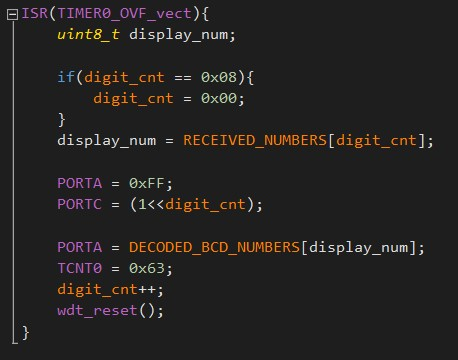
\includegraphics[height=3.5cm, width=\linewidth]{./results/lab6_timer0_changes.jpg}
			\caption{C code for WDT initilization}
		\end{subfigure}%
		~
		\begin{subfigure}[t]{0.5\textwidth}
			\centering
			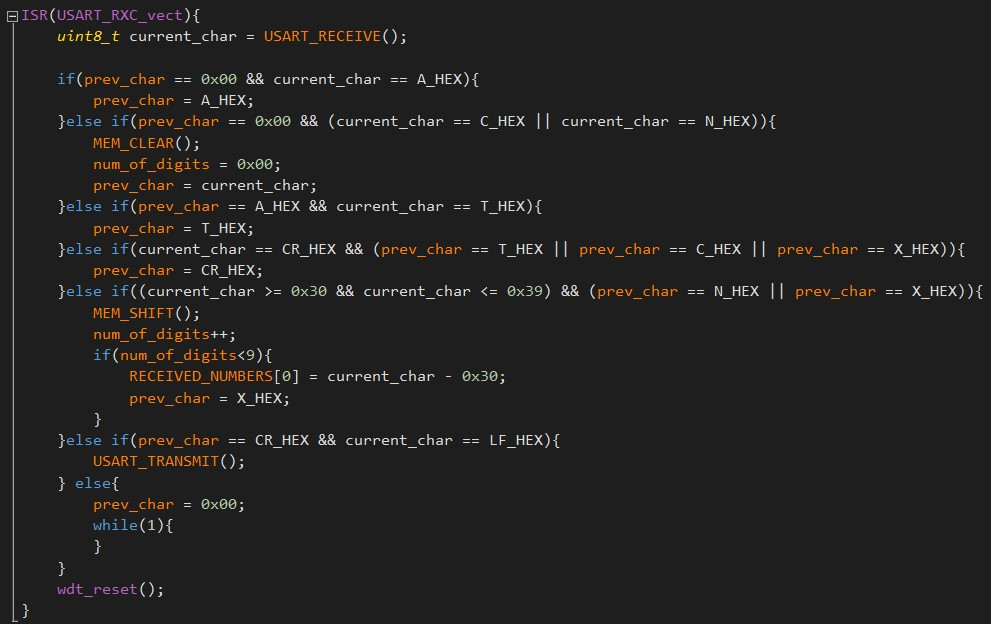
\includegraphics[height=3.5cm, width=\linewidth]{./results/lab6_usart_changes.jpg}
			\caption{C code for the changes in TIMER0 OVF Interrupt Handler}
		\end{subfigure}
	
		\begin{subfigure}[t]{0.5\textwidth}
			\centering
			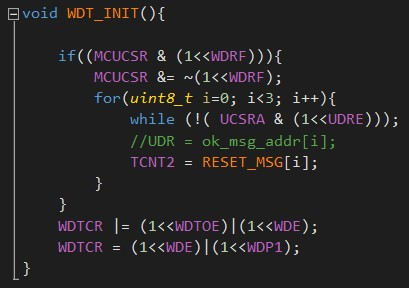
\includegraphics[height=3cm, width=\linewidth]{./results/lab6_wdt_init.jpg}
			\caption{C code for the changes in USART RXC Interrupt Handler}
		\end{subfigure}%
	\end{figure}

	\noindent
	\textbf{Προσομοίωση Αποτελεσμάτων} \\
	
	\noindent
	Aπό τα αποτελέσματα των προσομοιώσεων βλέπουμε ότι ο WDT αρχικοποιείται σωστά (εικόνα (a)). Στη επόμενη εικόνα βλέπουμε ότι λαμβάνουμε σωστά το ASCII code του χαρακτήρα C και αποθηκεύεται στη μνήμη. Επίσης, στην ίδια εικόνα φαίνεται ότι έχουμε μπει στo USART handler για τη λήψη του επόμενου χαρακτήρα της εντολής. \\
	
	\noindent
	Στις επόμενες δύο εικόνες βλέπουμε ότι το bit WDRF στον MCUCSR είναι "1", που σημαίνει ότι ξύπνησε ο WDT και έδωσε το reset. Επιπλέον, παρατηρούμε ότι όλα τα δεδομένα από τη μνήμη έχουν γίνει reset, κάτι το οποίο σημαίνει ότι έγινε cold start. Tέλος, βλέπουμε ότι γίνονται ξανά όλες οι αρχικοποιήσεις των καταχωρητών, καθώς και της το clear της μνήμης, όπως ήταν και κατα την πρώτη εκτέλεση του προγράμματος πριν το reset.\\
	
	\noindent
	Τέλος, στην τελευταία εικόνα βλέπουμε ότι μετά το reset και τη λήψη της λανθασμένης εντολής ο WDT δεν ξυπνάει μετά από περίπου 65000 κύκλους, καθώς τον κάνουμε reset μετά την ανανέωση των 7-segment LED. Συνεπώς, βλέπουμε ότι κάνουμε cold start μόνο όταν έρθει κάποια λάθος εντολή, ενώ στις υπόλοιπες περιπτώσεις διατηρούμε την κανονική λειτουργία του προγράμματος και τα δεδομένα στη μνήμη.
	
	\begin{figure}[h!]
		\centering
		\begin{subfigure}[t]{0.5\textwidth}
			\centering
			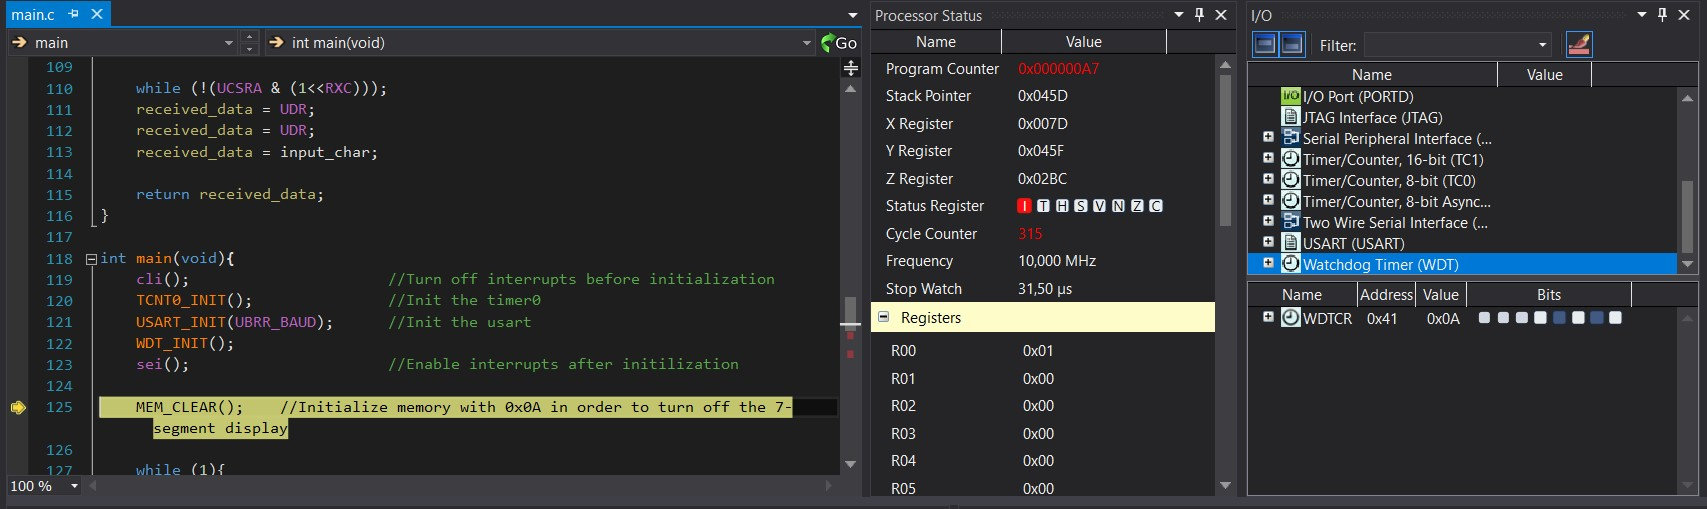
\includegraphics[height=3.5cm, width=\linewidth]{./results/lab6_sim_wdt_init.jpg}
			\caption{Αtmel Studio 7 - Initialization of WDT}
		\end{subfigure}%
		~
		\begin{subfigure}[t]{0.5\textwidth}
			\centering
			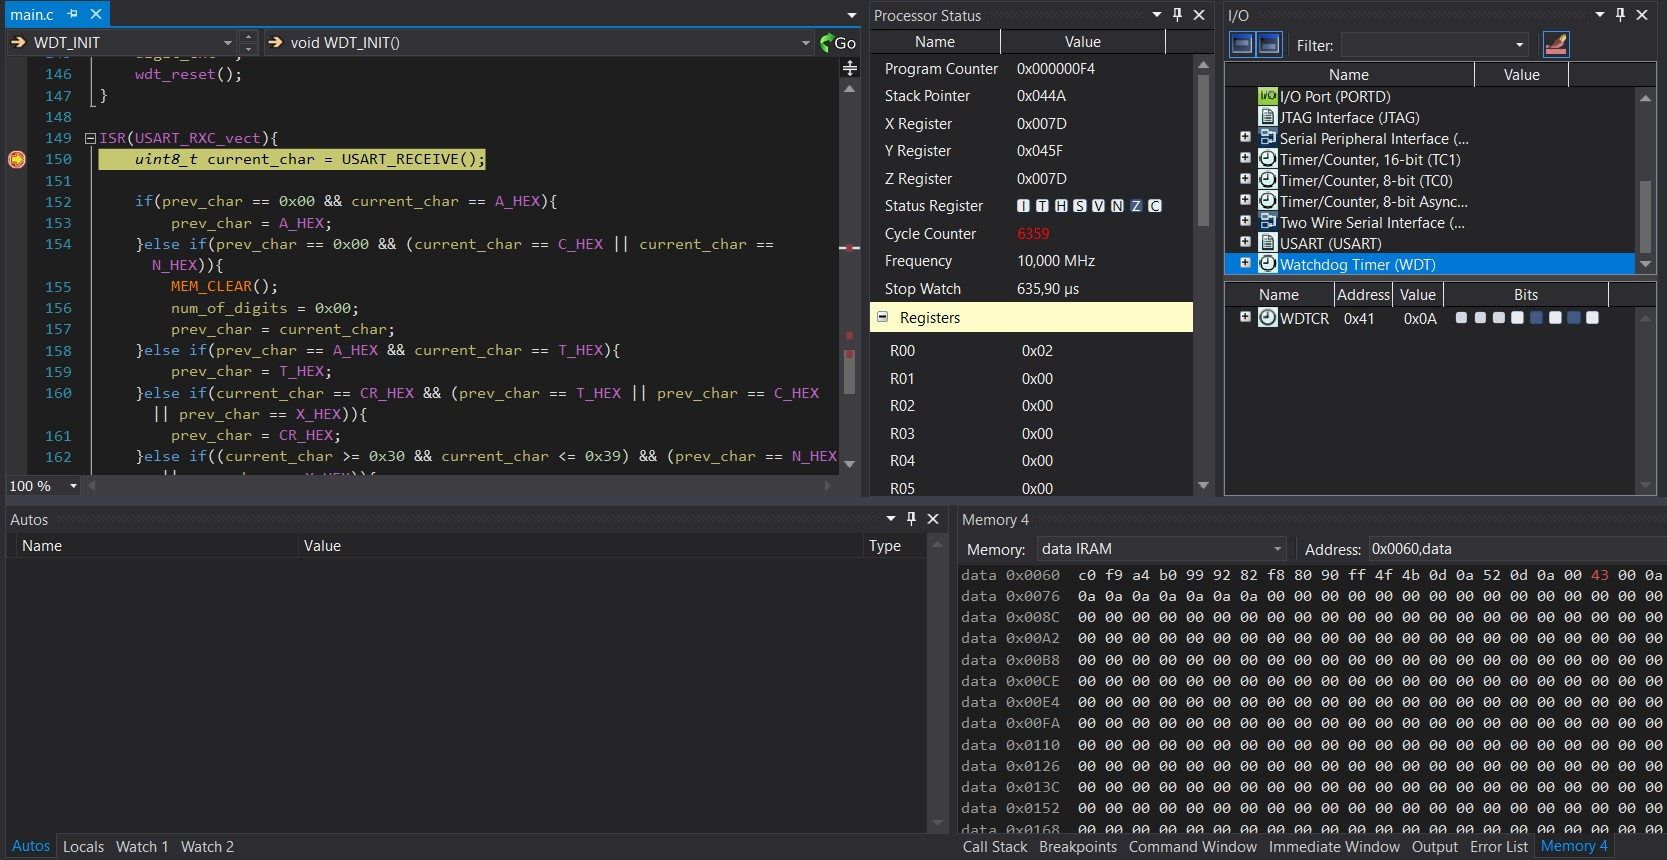
\includegraphics[height=3.5cm, width=\linewidth]{./results/lab6_sim_usart_rxc.jpg}
			\caption{Αtmel Studio 7 - Receive C from C<CR><LF> command}
		\end{subfigure}
	\end{figure}

\pagebreak
	\begin{figure}[h!]
		\centering
		\begin{subfigure}[t]{0.5\textwidth}
			\centering
			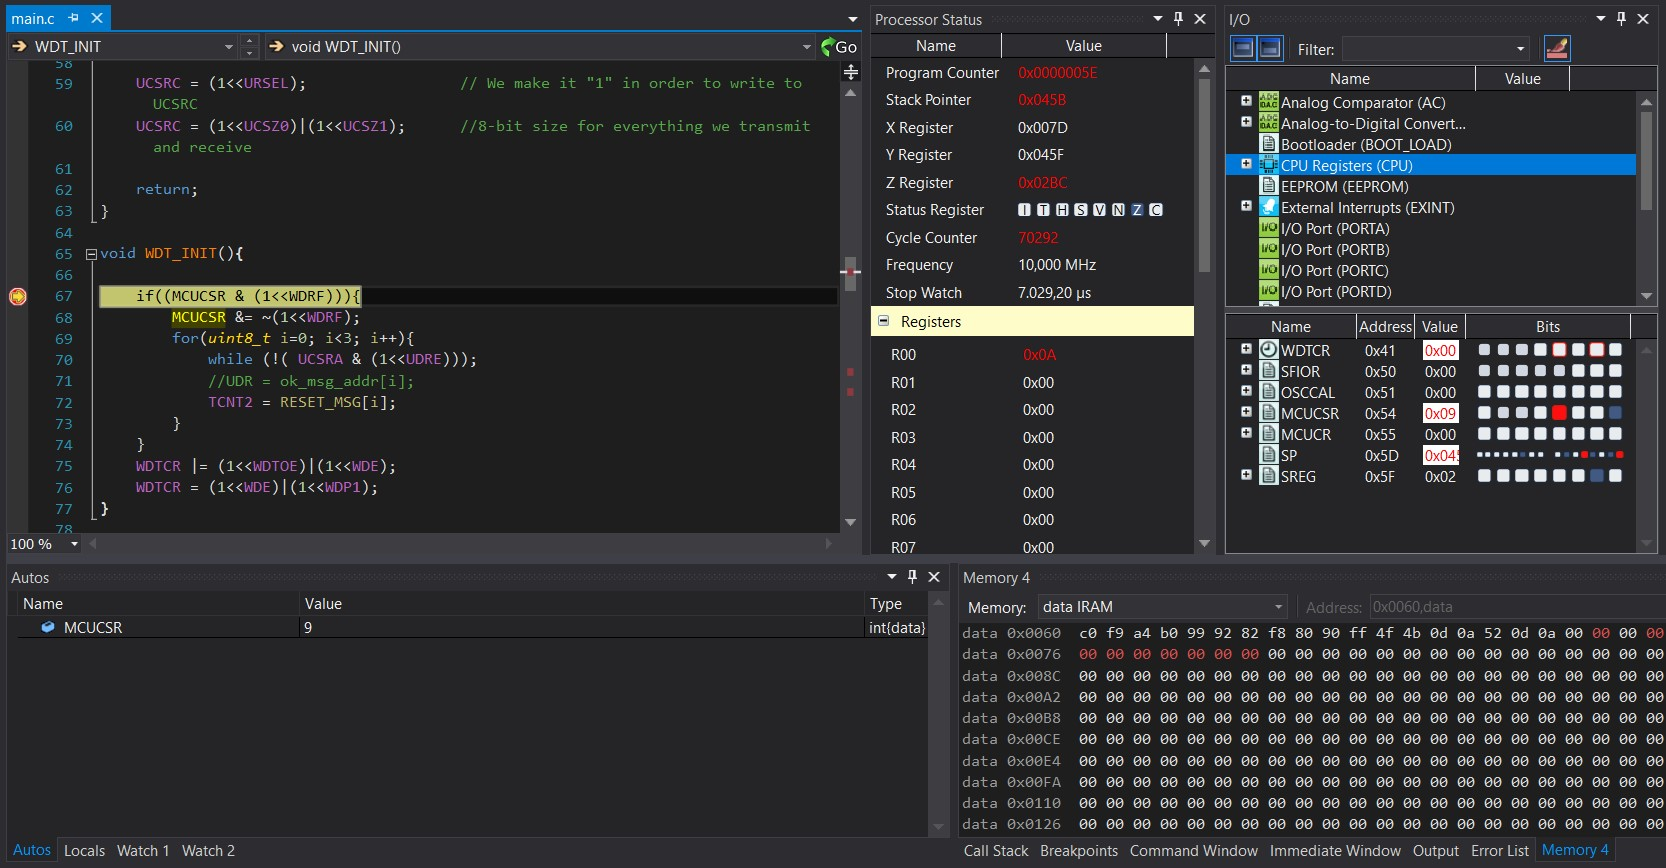
\includegraphics[height=3.5cm, width=\linewidth]{./results/lab6_sim_reset.jpg}
			\caption{Αtmel Studio 7 - WDT reset because of unknown ASCII character}
		\end{subfigure}%
		~
		\begin{subfigure}[t]{0.5\textwidth}
			\centering
			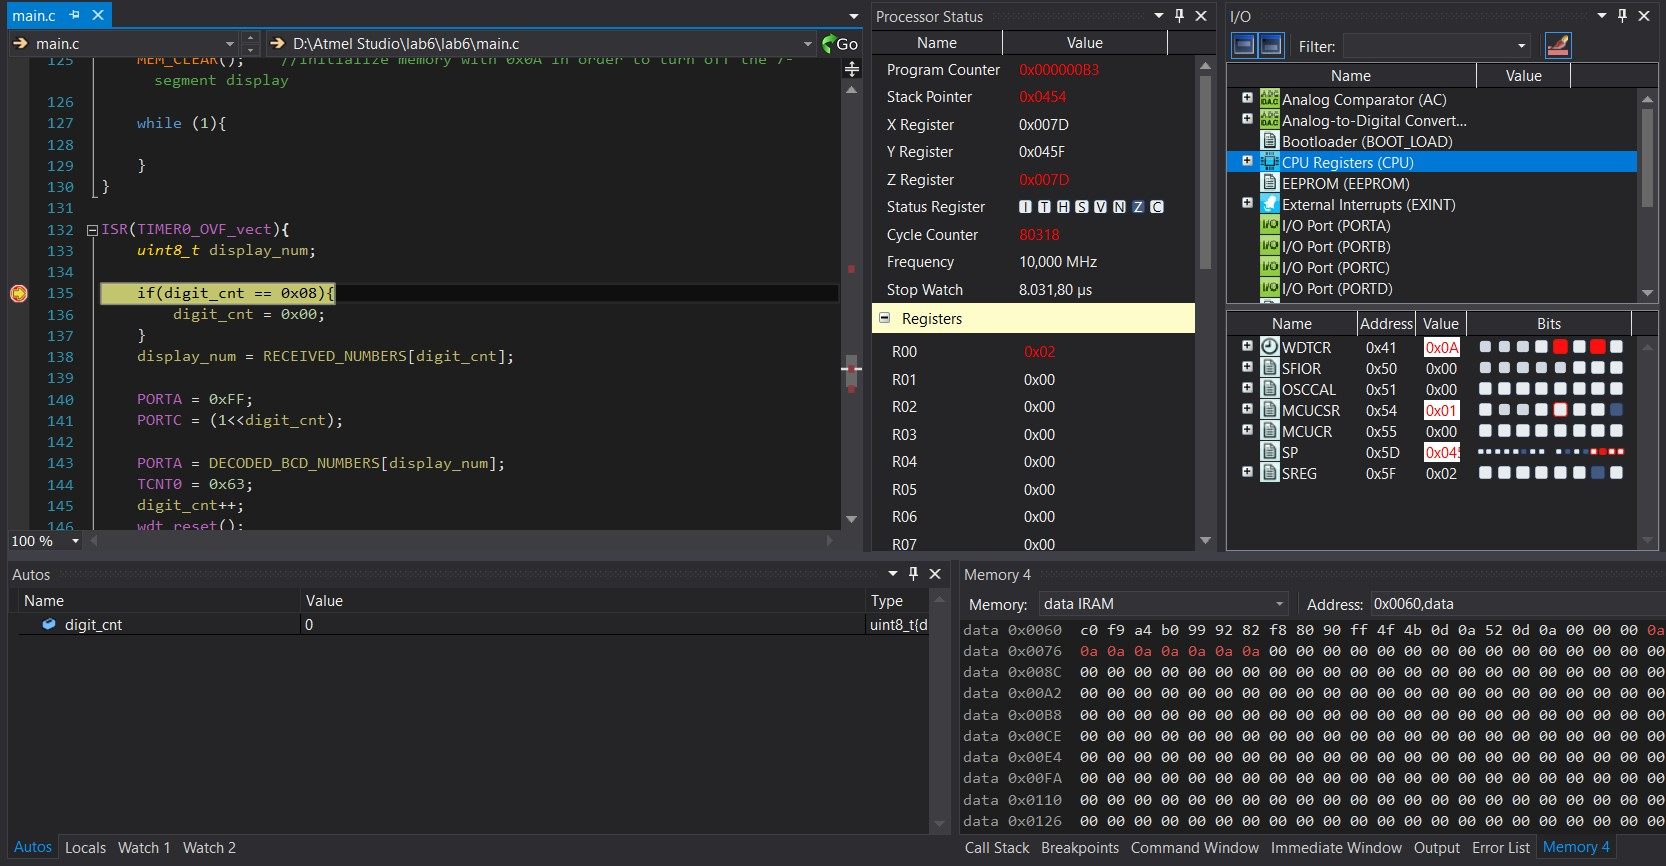
\includegraphics[height=3.5cm, width=\linewidth]{./results/lab6_sim_wdt_init_again.jpg}
			\caption{Αtmel Studio 7 - Initialize WDT once again}
		\end{subfigure}	
		\begin{subfigure}[t]{0.5\textwidth}
			\centering
			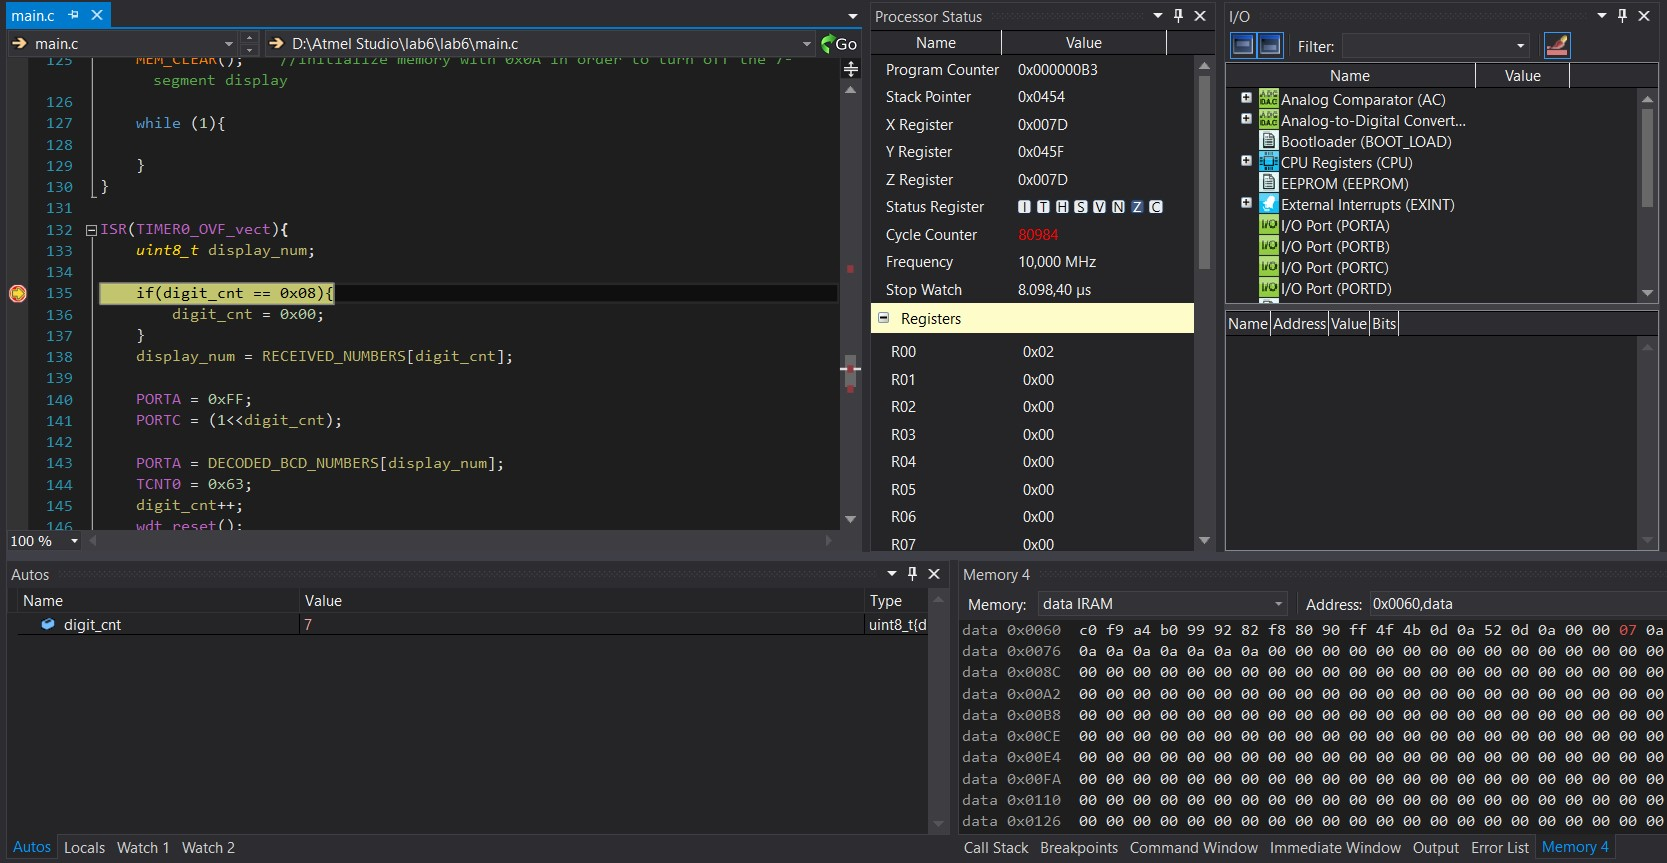
\includegraphics[height=3.5cm, width=\linewidth]{./results/lab6_sim_timer0.jpg}
			\caption{Αtmel Studio 7 - TIMER0 Interrupt Handler}
		\end{subfigure}	
	\end{figure}	
\end{document}
